\documentclass[10pt,a4paper]{article}
\usepackage[margin=20mm]{geometry}
\usepackage[T1]{fontenc}
\usepackage{lmodern,microtype,graphicx,booktabs,tabularx,xcolor}
\usepackage[hidelinks,pdftitle={Pet Care: Technical Brief Report},pdfauthor={}]{hyperref}
\definecolor{ink}{HTML}{234132}
\usepackage{titlesec}
\titleformat{\section}{\large\bfseries\color{ink}}{}{0pt}{}
\titlespacing*{\section}{0pt}{12pt}{5pt}
\setlength{\parindent}{0pt}
\setlength{\parskip}{6pt}
\begin{document}
{\LARGE\bfseries\color{ink} Pet Care}\par
{\large Technical Brief Report}\par
{\small HY359 Web Programming \enspace|\enspace Java Servlets, JDBC, JavaScript, MySQL}
\vspace{6pt}

Pet Care is a web application that connects pet owners with pet keepers. Owners register pets and request bookings, keepers review requests, and an administrator views accounts and summary statistics. The engineering work combines browser forms, asynchronous requests, servlet sessions, and relational data access.

\section*{Application design}
The browser uses HTML forms, client-side validation, JavaScript, and jQuery. AJAX requests submit JSON inside form parameters to Java servlets. The servlets interpret those requests, call JDBC table helpers, and return JSON that the browser uses to update the visible page without a full reload.

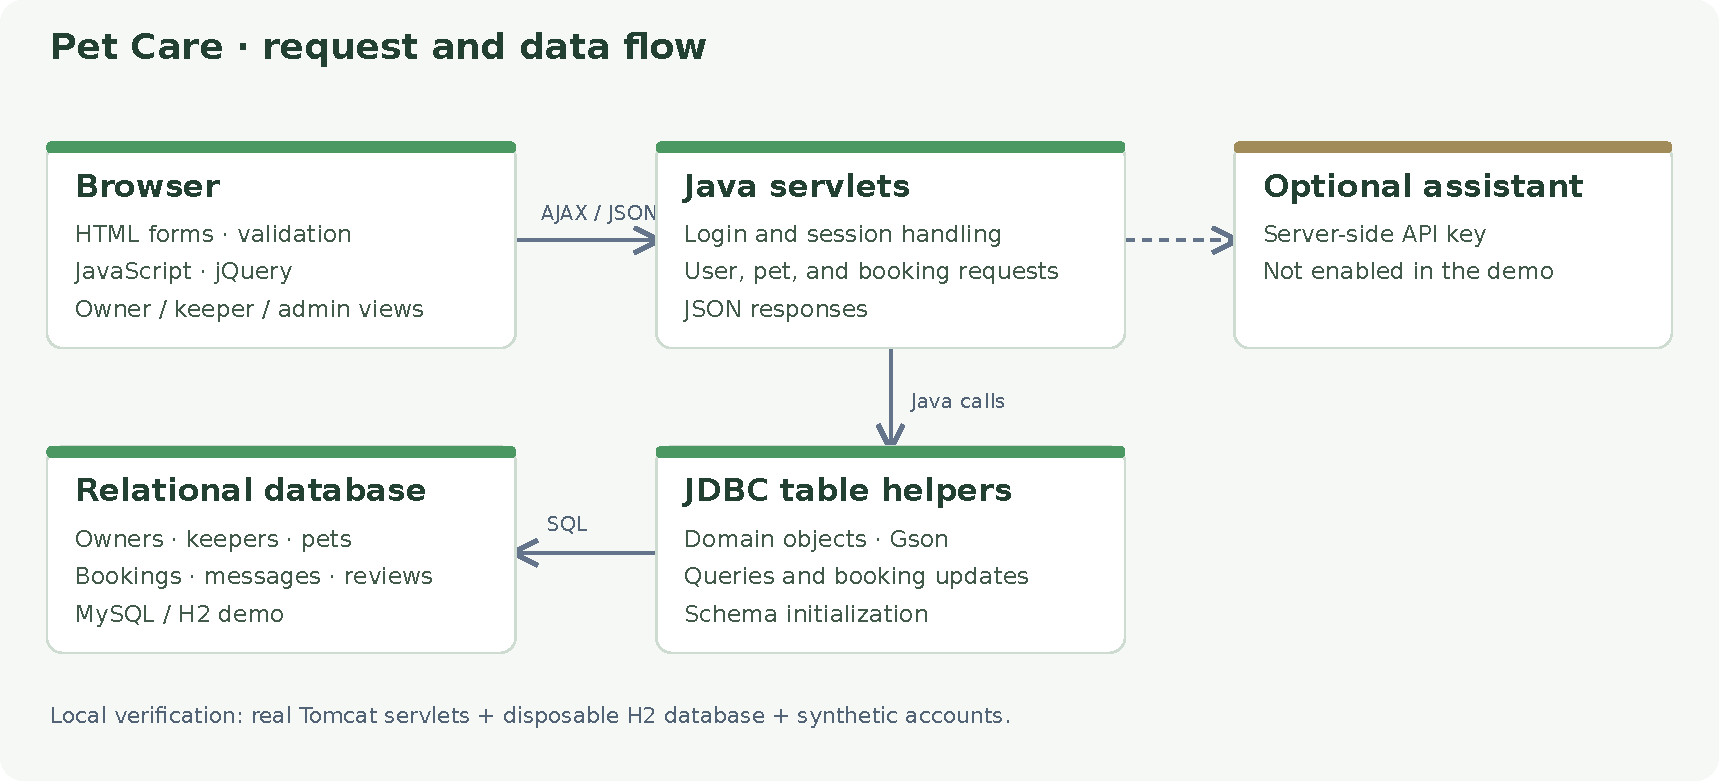
\includegraphics[width=\linewidth]{assets/architecture.pdf}

Login establishes an HTTP session. The returned session data selects an owner, keeper, or administrator view in the browser. The owner view queries keepers and supplies booking controls. The keeper view retrieves a requested booking and exposes accept/reject actions. The administrator view combines user records with counts and a share calculated from finished bookings.

\section*{Relational model}
Six tables hold owners, keepers, pets, bookings, messages, and reviews. A pet references its owner. A booking references an owner, pet, and keeper, together with dates, status, and price. Messages reference a booking, while reviews link an owner to a keeper.

Separating these records supports queries across the care workflow without storing the same booking inside every user record. Foreign keys enforce the main references. Domain objects and Gson convert database rows to JSON, while Jackson reads servlet request data.

Availability is based on booking status. Keepers with requested or accepted bookings are excluded from the unoccupied list across all dates. This is a simple occupancy rule rather than a date-overlap scheduler. The keeper's pending query currently returns one requested booking at a time.

\newpage
\section*{Booking and session flow}
An owner logs in, queries keepers, and submits a booking request. The stored record begins with a requested status. A keeper retrieves that request and sends an accepted or rejected response through a separate servlet. The status update changes the result of subsequent pending and availability queries.

This separation demonstrates a complete path from browser event to HTTP request, SQL update, and refreshed data. The current implementation does not enforce a complete booking state machine or protect every transition with server-side identity checks. Those are distinct requirements beyond displaying different role controls.

\section*{Reproducible local execution}
The Maven project builds a WAR for the \texttt{javax.servlet} API. A local demo starts the real application in embedded Tomcat with an isolated H2 database in MySQL compatibility mode. Synthetic fixtures provide one owner, three keepers, two pets, a requested booking, and a finished booking. No MySQL server or external API credential is required for the demo.

\renewcommand{\arraystretch}{1.25}
\begin{tabularx}{\linewidth}{@{}p{0.26\linewidth}X@{}}
\toprule
Evidence & Observed behavior \\
\midrule
HTTP/JDBC checks & Eight tests cover the directory, login/logout, rejected login, pending booking, availability, admin totals, key constraints, and disabled maintenance/API routes. \\
Browser interaction & Directory, administrator, and keeper views are captured from the running application. Accepting the requested booking removes it from the pending query. \\
Synthetic totals & The administrator sees one owner and three keepers. A finished booking priced at 30 produces a keeper share of 25.5 using the source's 85\% calculation. \\
Reproduction & \texttt{mvn verify} builds and checks the application. \texttt{mvn -Pdemo test-compile exec:java} starts the local demo. \\
\bottomrule
\end{tabularx}

The checks establish behavior under H2 and embedded Tomcat. They do not establish a MySQL deployment, external assistant availability, map integration, or every registration and profile-edit path. Screenshots use fictional accounts and no mocked server responses.

\section*{Implementation scope}
The source demonstrates servlet integration, relational queries, AJAX-driven views, and booking status updates. Messaging and review storage exist, but the current interface does not expose complete workflows for them. The map integration remains unfinished, and the optional assistant is disabled during verification.

The prototype uses concatenated SQL and plain passwords, returns broad account data, and relies on incomplete server-side authorization. Completing it would require prepared statements, secure password handling, session-bound identity checks, transaction rules, and broader workflow validation. Detailed setup and implementation boundaries are in \texttt{docs/SETUP.md}. The original course reports document the two submitted implementations.
\end{document}
